% GNUPLOT: LaTeX picture with Postscript
\begingroup
  \makeatletter
  \providecommand\color[2][]{%
    \GenericError{(gnuplot) \space\space\space\@spaces}{%
      Package color not loaded in conjunction with
      terminal option `colourtext'%
    }{See the gnuplot documentation for explanation.%
    }{Either use 'blacktext' in gnuplot or load the package
      color.sty in LaTeX.}%
    \renewcommand\color[2][]{}%
  }%
  \providecommand\includegraphics[2][]{%
    \GenericError{(gnuplot) \space\space\space\@spaces}{%
      Package graphicx or graphics not loaded%
    }{See the gnuplot documentation for explanation.%
    }{The gnuplot epslatex terminal needs graphicx.sty or graphics.sty.}%
    \renewcommand\includegraphics[2][]{}%
  }%
  \providecommand\rotatebox[2]{#2}%
  \@ifundefined{ifGPcolor}{%
    \newif\ifGPcolor
    \GPcolortrue
  }{}%
  \@ifundefined{ifGPblacktext}{%
    \newif\ifGPblacktext
    \GPblacktexttrue
  }{}%
  % define a \g@addto@macro without @ in the name:
  \let\gplgaddtomacro\g@addto@macro
  % define empty templates for all commands taking text:
  \gdef\gplbacktext{}%
  \gdef\gplfronttext{}%
  \makeatother
  \ifGPblacktext
    % no textcolor at all
    \def\colorrgb#1{}%
    \def\colorgray#1{}%
  \else
    % gray or color?
    \ifGPcolor
      \def\colorrgb#1{\color[rgb]{#1}}%
      \def\colorgray#1{\color[gray]{#1}}%
      \expandafter\def\csname LTw\endcsname{\color{white}}%
      \expandafter\def\csname LTb\endcsname{\color{black}}%
      \expandafter\def\csname LTa\endcsname{\color{black}}%
      \expandafter\def\csname LT0\endcsname{\color[rgb]{1,0,0}}%
      \expandafter\def\csname LT1\endcsname{\color[rgb]{0,1,0}}%
      \expandafter\def\csname LT2\endcsname{\color[rgb]{0,0,1}}%
      \expandafter\def\csname LT3\endcsname{\color[rgb]{1,0,1}}%
      \expandafter\def\csname LT4\endcsname{\color[rgb]{0,1,1}}%
      \expandafter\def\csname LT5\endcsname{\color[rgb]{1,1,0}}%
      \expandafter\def\csname LT6\endcsname{\color[rgb]{0,0,0}}%
      \expandafter\def\csname LT7\endcsname{\color[rgb]{1,0.3,0}}%
      \expandafter\def\csname LT8\endcsname{\color[rgb]{0.5,0.5,0.5}}%
    \else
      % gray
      \def\colorrgb#1{\color{black}}%
      \def\colorgray#1{\color[gray]{#1}}%
      \expandafter\def\csname LTw\endcsname{\color{white}}%
      \expandafter\def\csname LTb\endcsname{\color{black}}%
      \expandafter\def\csname LTa\endcsname{\color{black}}%
      \expandafter\def\csname LT0\endcsname{\color{black}}%
      \expandafter\def\csname LT1\endcsname{\color{black}}%
      \expandafter\def\csname LT2\endcsname{\color{black}}%
      \expandafter\def\csname LT3\endcsname{\color{black}}%
      \expandafter\def\csname LT4\endcsname{\color{black}}%
      \expandafter\def\csname LT5\endcsname{\color{black}}%
      \expandafter\def\csname LT6\endcsname{\color{black}}%
      \expandafter\def\csname LT7\endcsname{\color{black}}%
      \expandafter\def\csname LT8\endcsname{\color{black}}%
    \fi
  \fi
    \setlength{\unitlength}{0.0500bp}%
    \ifx\gptboxheight\undefined%
      \newlength{\gptboxheight}%
      \newlength{\gptboxwidth}%
      \newsavebox{\gptboxtext}%
    \fi%
    \setlength{\fboxrule}{0.5pt}%
    \setlength{\fboxsep}{1pt}%
\begin{picture}(10060.00,7180.00)%
      \csname LTb\endcsname%%
      \put(5030,6976){\makebox(0,0){\strut{}NaI case study}}%
    \gplgaddtomacro\gplbacktext{%
      \colorrgb{0.50,0.50,0.50}%%
      \put(336,3682){\makebox(0,0)[r]{\strut{}$0$}}%
      \colorrgb{0.50,0.50,0.50}%%
      \put(336,4040){\makebox(0,0)[r]{\strut{}$0.02$}}%
      \colorrgb{0.50,0.50,0.50}%%
      \put(336,4399){\makebox(0,0)[r]{\strut{}$0.04$}}%
      \colorrgb{0.50,0.50,0.50}%%
      \put(336,4757){\makebox(0,0)[r]{\strut{}$0.06$}}%
      \colorrgb{0.50,0.50,0.50}%%
      \put(336,5115){\makebox(0,0)[r]{\strut{}$0.08$}}%
      \colorrgb{0.50,0.50,0.50}%%
      \put(336,5473){\makebox(0,0)[r]{\strut{}$0.1$}}%
      \colorrgb{0.50,0.50,0.50}%%
      \put(336,5832){\makebox(0,0)[r]{\strut{}$0.12$}}%
      \colorrgb{0.50,0.50,0.50}%%
      \put(336,6190){\makebox(0,0)[r]{\strut{}$0.14$}}%
      \colorrgb{0.50,0.50,0.50}%%
      \put(336,6548){\makebox(0,0)[r]{\strut{}$0.16$}}%
      \colorrgb{0.50,0.50,0.50}%%
      \put(448,3478){\makebox(0,0){\strut{} }}%
      \colorrgb{0.50,0.50,0.50}%%
      \put(965,3478){\makebox(0,0){\strut{} }}%
      \colorrgb{0.50,0.50,0.50}%%
      \put(1481,3478){\makebox(0,0){\strut{} }}%
      \colorrgb{0.50,0.50,0.50}%%
      \put(1998,3478){\makebox(0,0){\strut{} }}%
      \colorrgb{0.50,0.50,0.50}%%
      \put(2515,3478){\makebox(0,0){\strut{} }}%
      \colorrgb{0.50,0.50,0.50}%%
      \put(3031,3478){\makebox(0,0){\strut{} }}%
      \colorrgb{0.50,0.50,0.50}%%
      \put(3548,3478){\makebox(0,0){\strut{} }}%
      \colorrgb{0.50,0.50,0.50}%%
      \put(4064,3478){\makebox(0,0){\strut{} }}%
      \colorrgb{0.50,0.50,0.50}%%
      \put(4581,3478){\makebox(0,0){\strut{} }}%
    }%
    \gplgaddtomacro\gplfronttext{%
      \csname LTb\endcsname%%
      \put(2418,3916){\makebox(0,0)[r]{\strut{}$\psi^+(x)$}}%
    }%
    \gplgaddtomacro\gplbacktext{%
      \colorrgb{0.50,0.50,0.50}%%
      \put(5366,3682){\makebox(0,0)[r]{\strut{}$0$}}%
      \colorrgb{0.50,0.50,0.50}%%
      \put(5366,4000){\makebox(0,0)[r]{\strut{}$1$}}%
      \colorrgb{0.50,0.50,0.50}%%
      \put(5366,4319){\makebox(0,0)[r]{\strut{}$2$}}%
      \colorrgb{0.50,0.50,0.50}%%
      \put(5366,4637){\makebox(0,0)[r]{\strut{}$3$}}%
      \colorrgb{0.50,0.50,0.50}%%
      \put(5366,4956){\makebox(0,0)[r]{\strut{}$4$}}%
      \colorrgb{0.50,0.50,0.50}%%
      \put(5366,5274){\makebox(0,0)[r]{\strut{}$5$}}%
      \colorrgb{0.50,0.50,0.50}%%
      \put(5366,5593){\makebox(0,0)[r]{\strut{}$6$}}%
      \colorrgb{0.50,0.50,0.50}%%
      \put(5366,5911){\makebox(0,0)[r]{\strut{}$7$}}%
      \colorrgb{0.50,0.50,0.50}%%
      \put(5366,6230){\makebox(0,0)[r]{\strut{}$8$}}%
      \colorrgb{0.50,0.50,0.50}%%
      \put(5366,6548){\makebox(0,0)[r]{\strut{}$9$}}%
      \colorrgb{0.50,0.50,0.50}%%
      \put(5891,3478){\makebox(0,0){\strut{} }}%
      \colorrgb{0.50,0.50,0.50}%%
      \put(6718,3478){\makebox(0,0){\strut{} }}%
      \colorrgb{0.50,0.50,0.50}%%
      \put(7545,3478){\makebox(0,0){\strut{} }}%
      \colorrgb{0.50,0.50,0.50}%%
      \put(8371,3478){\makebox(0,0){\strut{} }}%
      \colorrgb{0.50,0.50,0.50}%%
      \put(9198,3478){\makebox(0,0){\strut{} }}%
    }%
    \gplgaddtomacro\gplfronttext{%
      \csname LTb\endcsname%%
      \put(7504,3916){\makebox(0,0)[r]{\strut{}$\hat{\psi}^+(k)$}}%
    }%
    \gplgaddtomacro\gplbacktext{%
      \colorrgb{0.50,0.50,0.50}%%
      \put(336,408){\makebox(0,0)[r]{\strut{}$0$}}%
      \colorrgb{0.50,0.50,0.50}%%
      \put(336,704){\makebox(0,0)[r]{\strut{}$0.01$}}%
      \colorrgb{0.50,0.50,0.50}%%
      \put(336,1000){\makebox(0,0)[r]{\strut{}$0.02$}}%
      \colorrgb{0.50,0.50,0.50}%%
      \put(336,1295){\makebox(0,0)[r]{\strut{}$0.03$}}%
      \colorrgb{0.50,0.50,0.50}%%
      \put(336,1591){\makebox(0,0)[r]{\strut{}$0.04$}}%
      \colorrgb{0.50,0.50,0.50}%%
      \put(336,1887){\makebox(0,0)[r]{\strut{}$0.05$}}%
      \colorrgb{0.50,0.50,0.50}%%
      \put(336,2183){\makebox(0,0)[r]{\strut{}$0.06$}}%
      \colorrgb{0.50,0.50,0.50}%%
      \put(336,2478){\makebox(0,0)[r]{\strut{}$0.07$}}%
      \colorrgb{0.50,0.50,0.50}%%
      \put(336,2774){\makebox(0,0)[r]{\strut{}$0.08$}}%
      \colorrgb{0.50,0.50,0.50}%%
      \put(336,3070){\makebox(0,0)[r]{\strut{}$0.09$}}%
      \colorrgb{0.50,0.50,0.50}%%
      \put(448,204){\makebox(0,0){\strut{}8}}%
      \colorrgb{0.50,0.50,0.50}%%
      \put(965,204){\makebox(0,0){\strut{}9}}%
      \colorrgb{0.50,0.50,0.50}%%
      \put(1481,204){\makebox(0,0){\strut{}10}}%
      \colorrgb{0.50,0.50,0.50}%%
      \put(1998,204){\makebox(0,0){\strut{}11}}%
      \colorrgb{0.50,0.50,0.50}%%
      \put(2515,204){\makebox(0,0){\strut{}12}}%
      \colorrgb{0.50,0.50,0.50}%%
      \put(3031,204){\makebox(0,0){\strut{}13}}%
      \colorrgb{0.50,0.50,0.50}%%
      \put(3548,204){\makebox(0,0){\strut{}14}}%
      \colorrgb{0.50,0.50,0.50}%%
      \put(4064,204){\makebox(0,0){\strut{}15}}%
      \colorrgb{0.50,0.50,0.50}%%
      \put(4581,204){\makebox(0,0){\strut{}16}}%
    }%
    \gplgaddtomacro\gplfronttext{%
      \csname LTb\endcsname%%
      \put(2250,642){\makebox(0,0)[r]{\strut{}$\psi^-$}}%
    }%
    \gplgaddtomacro\gplbacktext{%
      \colorrgb{0.50,0.50,0.50}%%
      \put(5366,408){\makebox(0,0)[r]{\strut{}$0$}}%
      \colorrgb{0.50,0.50,0.50}%%
      \put(5366,674){\makebox(0,0)[r]{\strut{}$0.5$}}%
      \colorrgb{0.50,0.50,0.50}%%
      \put(5366,940){\makebox(0,0)[r]{\strut{}$1$}}%
      \colorrgb{0.50,0.50,0.50}%%
      \put(5366,1207){\makebox(0,0)[r]{\strut{}$1.5$}}%
      \colorrgb{0.50,0.50,0.50}%%
      \put(5366,1473){\makebox(0,0)[r]{\strut{}$2$}}%
      \colorrgb{0.50,0.50,0.50}%%
      \put(5366,1739){\makebox(0,0)[r]{\strut{}$2.5$}}%
      \colorrgb{0.50,0.50,0.50}%%
      \put(5366,2005){\makebox(0,0)[r]{\strut{}$3$}}%
      \colorrgb{0.50,0.50,0.50}%%
      \put(5366,2271){\makebox(0,0)[r]{\strut{}$3.5$}}%
      \colorrgb{0.50,0.50,0.50}%%
      \put(5366,2538){\makebox(0,0)[r]{\strut{}$4$}}%
      \colorrgb{0.50,0.50,0.50}%%
      \put(5366,2804){\makebox(0,0)[r]{\strut{}$4.5$}}%
      \colorrgb{0.50,0.50,0.50}%%
      \put(5366,3070){\makebox(0,0)[r]{\strut{}$5$}}%
      \colorrgb{0.50,0.50,0.50}%%
      \put(5891,204){\makebox(0,0){\strut{}-0.40}}%
      \colorrgb{0.50,0.50,0.50}%%
      \put(6718,204){\makebox(0,0){\strut{}-0.20}}%
      \colorrgb{0.50,0.50,0.50}%%
      \put(7545,204){\makebox(0,0){\strut{}0.00}}%
      \colorrgb{0.50,0.50,0.50}%%
      \put(8371,204){\makebox(0,0){\strut{}0.20}}%
      \colorrgb{0.50,0.50,0.50}%%
      \put(9198,204){\makebox(0,0){\strut{}0.40}}%
    }%
    \gplgaddtomacro\gplfronttext{%
      \csname LTb\endcsname%%
      \put(7280,642){\makebox(0,0)[r]{\strut{}$\psi^-$}}%
    }%
    \gplbacktext
    \put(0,0){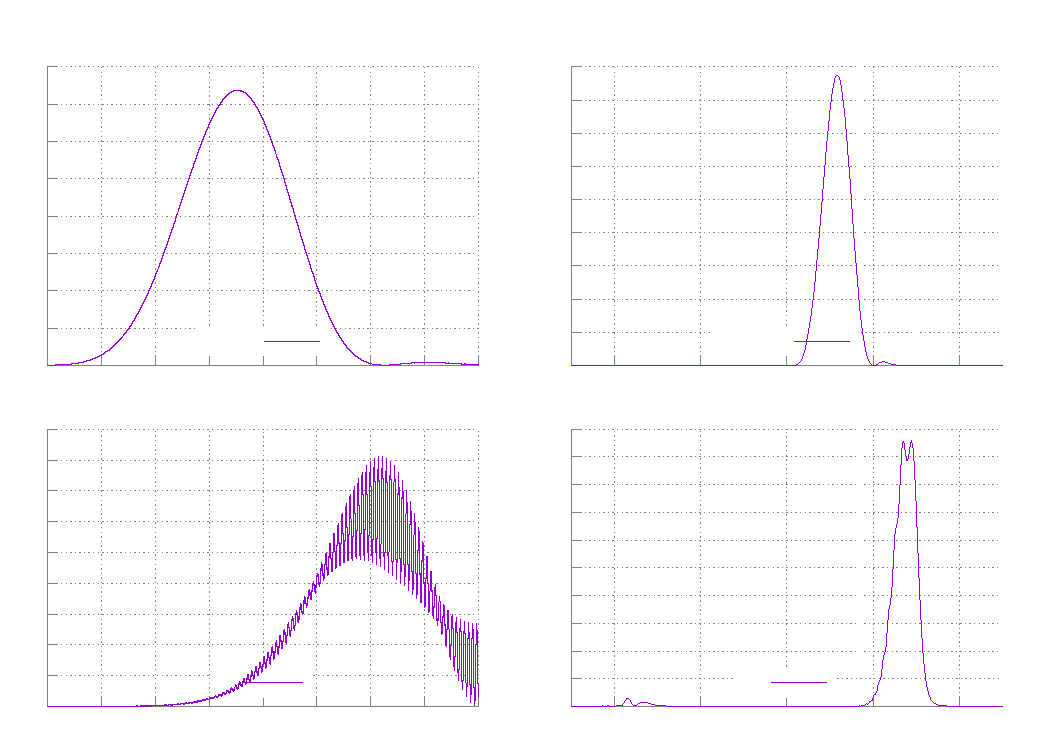
\includegraphics{/home/s1992054/QMD/src/nai/plots/nai_final_wavepacket}}%
    \gplfronttext
  \end{picture}%
\endgroup
